\documentclass[11pt]{article}
\usepackage{listings,amsmath,amssymb,bbm}
\usepackage{amsthm}
\usepackage{graphicx}
\usepackage{color}
\usepackage{multirow}
\usepackage{natbib}
\usepackage{algorithm}
\usepackage{algorithmic}
\oddsidemargin0cm
\topmargin-1.4cm
\textheight23.5cm
\textwidth16cm
%\parindent0cm
\renewcommand{\baselinestretch}{1.1}
\numberwithin{equation}{section}
\lstset{language=R,basicstyle=\ttfamily\footnotesize,breaklines=true}
\usepackage{booktabs}
\def\R{{\mathbb R}}  %%
\def\N{{\mathbb N}}  %%
\def\E{{\mathbb E}}  %%
\def\Z{{\mathbb Z}}  %%
\def\bc{\boldsymbol{c}}
\def\bd{\boldsymbol{d}}
\def\bx{\boldsymbol{x}}
\def\bm{\boldsymbol{m}}
\def\by{\boldsymbol{y}}
\def\bp{\boldsymbol{p}}
\def\bmu{\boldsymbol{\mu}}
\def\bphi{\boldsymbol{\phi}}
\def\bZ{\boldsymbol{Z}}
\def\bz{\boldsymbol{z}}

\newcounter{saveenumi}
\newcommand{\seti}{\setcounter{saveenumi}{\value{enumi}}}
\newcommand{\conti}{\setcounter{enumi}{\value{saveenumi}}}

\newcommand{\blue}[1]{\textcolor{blue}{#1}}
\newcommand{\red}[1]{\textcolor{red}{#1}}
\usepackage{url}%For ref url
%\bibliographystyle{plain}
%opening
\title{Insurance loss modelling with gradient tree-boosted mixture models}
\author{ Yanxi Hou\footnote{School of Data Science, Fudan University, 200433 Shanghai, China.} \and Jiahong Li\footnote{School of Mathematical Sciences, Peking University, 100871 Beijing, China.} \and Guangyuan Gao\footnote{Center for Applied Statistics and School of Statistics, Renmin University of China, 100872 Beijing, China.}}


\begin{document}

\maketitle

\begin{abstract}
%Insurance loss data always cannot be well modeled by a single distribution.
\noindent 
In actuarial practice, mixture models {\color{blue}[mixture models or mixture of models? both appear in the paper]} is one widely applied statistical method to model the insurance loss data. 
Although the Expectation-Maximization (EM) algorithm usually plays an important tool for the parameter estimation of mixture  models, it suffers from other issues which cause unstable predictions. 
For example, the feature engineering and variable selection are two important modelling issues, which are challenging for mixture models due to several component models involving. 
Moreover, to avoid overfitting is another technical concern of the modelling method for prediction of future losses. 
To address those issues, we propose an Expectation-Boosting (EB) algorithm, 
which replaces the maximization step in the EM algorithm by gradient boosting machines with decision trees. 
Our proposed EB algorithm can estimate the component regression functions non-paramerically and overfitting-sensitively, as well as
perform automated feature engineering, model fitting and variable selection simultaneously, which
fully explores the predictive power of feature space.
We also conduct two simulation studies to show the good performance of the proposed algorithm and an empirical analysis of the claims amounts data for illustration. 

\end{abstract}

{\bf Keywords:} Insurance loss; Mixture models; EM algorithm; Gradient boosting; Parallel computing; Finite mixture of regressions; Zero-inflated Poisson model. 


\section{Introduction}

It is well known that insurance loss data sometimes cannot be well modeled by a single distribution due to its complex data structures.
For claim count data, a Poisson distribution may not be the best choice to model an excess of zero claims.
For claim amount data, it usually exhibits multimodal or heavy-tailed phenomenons, so a gamma distribution is not sufficient to address these data features.
In the literature, one alternative way is to apply a mixture of distributions for univariate loss data.
When the individual risk factors are available, a mixture of regressions is then used instead to model the risk heterogeneity, which is an extension to the mixture of distributions. 
In the literature,
mixture models are proposed by \citet{goldfeld1973markov}.
We refer to \citet{lindsay1995mixture} and \citet{peel2000finite} for a detailed review of mixture models.
In the field of machine learning research, mixture models are also called as mixture of experts models \citep{jacobs1991adaptive,jiang1999hierarchical}.

We summarize some studies on mixture models for insurance loss modelling.
\citet{zhang2020type, zhang2022new} developed a multivariate zero-inflated hurdle model to describe multivariate count data with extra zeros.
\citet{delong2021gamma} proposed a mixture of neural networks with gamma loss to model insurance claim amounts.
\citet{lee2010modeling} and \citet{verbelen2015fitting} used a mixture of Erlangs to model insurance claim amounts including censored and truncated data.
\citet{lee2012modeling} developed the multivariate version of mixture of Erlangs.
\citet{fung2019class2}, \citet{fung2019class} and \citet{tseung2021lrmoe} proposed a so called logit-weighted reduced mixture of experts models for multivariate claim frequencies or severities distributions.
To the best of our knowledge, the existing studies always impose a linearity constraint on the regression function, i.e., under a generalized linear model (GLM) framework.
In this paper, we will relax this constraint by estimating regression functions non-parametrically.

Several aspects of modelling are very noteworthy in research. It is challenging to estimate parameters in mixture models, since the parameters in component models are related to each other.
To overcome it,  \citet{dempster1977maximum} proposed the Expectation-Maximization (EM) algorithm, which is an iterative method to estimate the component parameters and the latent component indicator variables. 
In addition, the variable selection and the feature engineering in mixture models are also challenging since the dependence between the covariate and response variables varies from one component to another.  
\citet{khalili2007variable} introduced a penalized likelihood approach for the variable selection.
\citet{huang2012mixture} and \citet{huang2013nonparametric} proposed a non-parametric mixture of regressions to relax the linearity assumption on the regression function.
Moreover, the selection of the number of the components is another challenging problem.
\citet{naik2007extending} derived a new information criterion for the selection of the component number and variables.
\citet{kasahara2015testing} proposed a likelihood-based test to contrast  the mixture models with different numbers of components. 
In this paper, we assume that the number of components is known, and we will address variable selection and feature engineering in the proposed method.

We propose an Expectation-Boosting (EB) algorithm for mixture models, which replaces the maximization step by a boosting step. 
It is well known that the boosting algorithm is an iterative method to estimate the regression function non-parametrically, where weak learners are calibrated step-wisely and added together.
We roughly categorize some commonly used boosting algorithms into three groups: 
(a) Binary classification: {AdaBoost}, LogitBoost (real, discrete, gentle AdaBoost), AdaBoost.M1; 
(b) Multinomial classification: Stagewise Additive Modelling using a Multi-class Exponential loss (SAMME), SAMME.R (multi-class real AdaBoost); 
(c) {Gradient based}: {gradient boosting machine/model (GBM)}, Newton boosting, gradient boosting decision tree (GBDT), {eXtreme Gradient Boosting (XGBoost)}, {light gradient boosting machine (LightGBM)}.
The last type is based on {gradient of loss function} and \citet{friedman2001greedy} has studied this type of boosting from a statistical perspective as an additive model.
Our EB algorithm follows the GBDT algorithm in the boosting step.
With the negative log-likelihood as the loss function for boosting, the boosting step increases the likelihood at each iteration of the EB algorithm. 
There are several advantages of the EB algorithm over the EM algorithm. 
First, the boosting algorithm is a flexible non-parametric regression method, which facilitates both non-linear effects and interaction. Thus, the variable selection and feature engineering are performed automatically during the model fitting. 
Second, it is well known that the boosting algorithm is overfitting-sensitive \citep{buehlmann:2003}. This property is very useful since the ultimate goal of insurance loss modelling is to predict the future loss. Therefore,
the out-of-sample prediction is more important than the goodness-of-fitting in our applications. 

%Boosting algorithm has a close relationship with the additive model.

The rest of paper is structured as follows. 
Section \ref{sec:review} reviews mixture models and the EM algorithm. 
Section \ref{sec:EB} presents the EB algorithm. We also discuss initialization, tuning parameters and parallel computing in detail.   
Section \ref{sec:application} studies two simulated data and a real data to illustrate the proposed methodology. Section \ref{sec:conclusions} concludes the paper with several important findings.  The R code of our work is publicly available on the github (\url{https://github.com/sxpyggy/boosting-mixture-code}).


\section{Review: mixture models and the EM algorithm}\label{sec:review}

In this section, we first review mixture models, particularly finite mixture of regressions \citep{peel2000finite}, and discuss different mixture structure. 
Then we review the EM algorithm which is the foundation of the proposed EB algorithm. 
In this paper, we focus on the exponential distribution family with an expectation parameter $\mu$ and a dispersion parameter $\phi$. 
The exponential distributions form a general family of parametric distributions, which are fitting for different types of insurance loss data.

\subsection{Mixture models}\label{review:mix1}
Suppose a random variable $y$ follows a finite mixture of distributions with the $k$-th {\it component distribution} from a finite collection of distributions
	$$\{f_1(y;\mu_1,\phi_1),\ldots,f_K(y;\mu_K,\phi_K)\}$$
	and \textit{mixing probability} $p_k, k=1,\ldots,K$($K \geqslant 1$).
	The probability density function for $y$ is given by a weighted sum of component distributions such that
	$$f(y)=\sum_{k=1}^Kp_kf_k(y;\mu_k,\phi_k).$$
	If the {\it individual features $\bx_i$} are available and have a systematic effect on the response variable $y_i$, then we can establish a finite mixture of regressions:
	\begin{equation}\label{mix-gen}
		f(y|\bx)=\sum_{k=1}^Kp_k(\bx)f_k(y|\bx;\mu_k(\bx),\phi_k(\bx)).
	\end{equation}
	Note that \eqref{mix-gen} is a general representation for a finite mixture of regressions, 
	i.e., both mixing probabilities and component parameters depend on $\bx$.
	 
	 In real applications,  based on the features of data and the goal of modelling, we can make specific assumptions on \eqref{mix-gen}. For example,
	\begin{itemize}
		\item The mixing probabilities are not related to $\bx$
		$$f(y|\bx)=\sum_{k=1}^Kp_kf_k(y|\bx;\mu_k(\bx),\phi_k(\bx));$$
		\item Both mixing probabilities and dispersions are not related to $\bx$
		$$f(y|\bx)=\sum_{k=1}^Kp_kf_k(y|\bx;\mu_k(\bx),\phi_k);$$

		\item If the component distributions are from the same distribution family, we might assume that different component distributions have the same dispersion $\phi$
		$$f(y|\bx)=\sum_{k=1}^Kp_kf_k(y|\bx;\mu_k(\bx),\phi);$$
		\item The covariates $\bx$ are only related to the mixing probabilities:
		$$f(y|\bx)=\sum_{k=1}^Kp_k(\bx)f_k(y;\mu_k,\phi_k).$$
	\end{itemize}
	Selection among the above model alternatives can be viewed as imposing suitable constraints on the general form \eqref{mix-gen}, which accelerates and stabilizes model fitting without compromising predictive performance. It actually provides practical flexibility according to different data structures and the goals of study.
	% However, the proposed EB algorithm can still {accelerate and stabilize model fitting} without compromising predictive performance.

\subsection{The EM algorithm}

	Suppose that for a single sample $y$, we know exactly which component distribution it comes from, that is, we know the \textit{full information} $(Y,\bZ,\bx)$, where
	$$\bZ=(Z_1,\ldots,Z_K)=(\mathbbm{1}_1(k),\ldots,\mathbbm{1}_K(k))$$
	is the one-hot encoding vector of \textit{component indicator variable $k$}.
	Then the joint distribution function of $(Y,\bZ)$ given $\bx$ is given by
	$$f(y,\bz|
	\bx) = \prod_{k=1}^K\left[p_k(\bx)f_k(y|\bx;\mu_k(\bx),\phi_k(\bx))\right]^{z_k}.$$
	Equivalently, the {complete log-likelihood function} is 
	\begin{equation}\label{full-L}
		l(p,\mu,\phi|y,\bz,\bx)=\sum_{k=1}^K z_k\left[\log p_k(\bx) + \log f_k(y|\bx;\mu_k(\bx),\phi_k(\bx))\right].
	\end{equation}
	 Given a data set $\{(y_i,\bz_i,\bx_i)\}_{i=1:n}$, we assume the parametric models of $p=(p_1,\ldots,p_K),\mu_k,\phi_k$ such that $p(\bx)=(p_1(\bx;\theta_p),\ldots,p_K(\bx;\theta_p))$, $\mu_k(\bx)=\mu_k(\bx;\theta_\mu^{(k)})$ and $\phi_k(\bx)=\phi_k(\bx;\theta_\phi^{(k)})$, where $\theta_p, (\theta_\mu^{(k)})_{k=1:K}, (\theta_\phi^{(k)})_{k=1:K}$ are the unknown parameters. Note that $\theta_p$ does not have a superscript since it corresponds to coefficients in a multinomial logistic classification while $\theta_\mu^{(k)},\theta_\phi^{(k)}$ can be considered in separate component models; see below.
	 
	 The regression coefficients can be estimated by the following $K+1$ {independent optimizations:}
	\begin{equation}\label{p-reg}
		\hat{\theta}_p=\underset{\theta_p}{\arg\max}\sum_{i=1}^n\sum_{k=1}^Kz_{i,k}\log p_k(\bx_i;\theta_p)
	\end{equation}
and
	\begin{equation}\label{comp-reg}
		\left(\hat{\theta}_\mu^{(k)},\hat{\theta}_\phi^{(k)}\right)=\underset{\theta^{(k)}_\mu,\theta^{(k)}_\phi}{\arg\max}\sum_{i=1}^n\sum_{k=1}^Kz_{i,k}\log f_k\left(y_i;\mu_k\left(\bx_i;\theta_\mu^{(k)}\right),\phi_k\left(\bx_i;\theta_\phi^{(k)}\right)\right), ~\text{for} ~ k=1,\ldots,K.
	\end{equation}
	Those optimizations are corresponding to  {\it a multinomial logistic classification} and {\it $K$ regressions}.
The multinomial logistic classification \eqref{p-reg} are fitted to all samples, while the $k$-th regression in \eqref{comp-reg} is fitted to {partial} samples with $\{i:z_{i,k}=1\}$.
In practice we do not have the full information  $(Y,\bZ,\bx)$, but only the incomplete information $(Y,\bx)$. The EM algorithm is inspired by the above discussion.
\paragraph{Expectation step.}
	With iterated $\hat{p},\hat{\mu},\hat{\phi}$, calculate the \textit{conditional expectation} of $\bz$:
	$$\hat{z}_{i,k}=\hat{z}_k(\bx_i)=\frac{\hat{p}_{i,k}f_k(y_i;\hat{\mu}_{i,k},\hat{\phi}_{i,k})}{\sum_{l=1}^K\hat{p}_{i,l}f_l(y_i;\hat{\mu}_{i,l},\hat{\phi}_{i,l})},$$
	where
	$\hat{p}_{i,k}=\hat{p}_k(\bx_i)= p_k(\bx_i;\hat{\theta}_p),\hat{\mu}_{i,k}=\hat{\mu}_k(\bx_i)=\mu_k\left(\bx_i;\hat{\theta}_\mu^{(k)}\right),\hat{\phi}_{i,k}=\hat{\phi}_k(\bx_i)=\phi_k\left(\bx_i;\hat{\theta}_\phi^{(k)}\right)$.

\paragraph{Maximization step.}
	Based on the log-likelihood function for full information
	\begin{equation}\label{likelihood}
		\begin{aligned}
			&l(p,\mu,\phi|\by,\hat{\bz},\bx)\\
			=&\sum_{i=1}^n\sum_{k=1}^K \hat{z}_{i,k}\left[\log p_k(\bx_i;\theta_p) + \log f_k\left(y_i;\mu_k\left(\bx_i;\theta_\mu^{(k)}\right),\phi_k\left(\bx_i;\theta_\phi^{(k)}\right)\right)\right]\\
			=&\sum_{i=1}^n\sum_{k=1}^K \hat{z}_{i,k}\log p_k(\bx_i;\theta_p) + \sum_{i=1}^n\sum_{k=1}^K \hat{z}_{i,k}\log f_k\left(y_i;\mu_k\left(\bx_i;\theta_\mu^{(k)}\right),\phi_k\left(\bx_i;\theta_\phi^{(k)}\right)\right),
		\end{aligned}
	\end{equation}
 calculate the MLE of regression coefficients by the following $K+1$ independent optimizations:
 	\begin{equation}\label{p-reg2}
 	\hat{\theta}_p=\underset{\theta_p}{\arg\max}\sum_{i=1}^n\sum_{k=1}^K\hat{z}_{i,k}\log p_k(\bx_i;\theta_p)
 \end{equation}
 and
 \begin{equation}\label{comp-reg2}
 	\left(\hat{\theta}_\mu^{(k)},\hat{\theta}_\phi^{(k)}\right)=\underset{\theta^{(k)}_\mu,\theta^{(k)}_\phi}{\arg\max}\sum_{i=1}^n\sum_{k=1}^K\hat{z}_{i,k}\log f_k\left(y_i;\mu_k\left(\bx_i;\theta_\mu^{(k)}\right),\phi_k\left(\bx_i;\theta_\phi^{(k)}\right)\right), ~\text{for} ~ k=1,\ldots,K.
 \end{equation}
{\color{blue}[why using bold $\bp,\bmu,\bphi,\by$? Need to define some new notions above?]} These optimizations are similar to those in \eqref{p-reg} and \eqref{comp-reg}. 
The only difference is that ${z}_{i,k}\in\{0,1\}$ in \eqref{p-reg} and \eqref{comp-reg} while $\hat{z}_{i,k}\in(0,1)$ in  \eqref{p-reg2} and \eqref{comp-reg2}.
Therefore, in the maximization step we perform a multinomial logistic classification with {\it fractional} response $\hat{z}_{i,k}$ {\color{blue}[No illustration for a fractional response]} and $K$ {weighted}-regressions {\color{blue}[No illustration as well]} fitted to {\it all} samples with weights $\hat{z}_{i,k}$.

\section{Expectation-Boosting algorithm}\label{sec:EB}
In the EM algorithm, the functions $p(\bx), \mu_k(\bx), \phi_k(\bx)$ are always assumed to be parametric functions.
To make component models more flexible, we replace the maximization step in the EM algorithm by a boosting step.
Boosting algorithm estimates the regression functions non-parametrically and facilitates more flexible shapes of regression function.
With negative log-likelihood function as the loss function in boosting algorithm, the boosting step increases the likelihood at each iteration, but overfitting-sensitively.
The boosting step follows a generic functional gradient descent algorithm.
We first describe generic functional gradient descent algorithm, then propose the EB algorithm. {\color{blue}[why not put the review of generic functional gradient descent algorithm in Section 2.]}

\subsection{Generic functional gradient descent algorithm}

	Suppose a to-be-boosted {non-parametric regression function} as $F:\R^P\rightarrow\R$. In boosting algorithm, the goal is to  estimate $F$ to minimize the expected loss $$\hat{F}=\underset{F}{\arg\min}\E\left[C(Y,F(\bx))\right],$$
	where $C:\R\times\R\rightarrow\R_+$ is the \textit{loss function}.
	The expected loss is always replaced by sample average loss:
	$$\hat{F}=\underset{F}{\arg\min}\frac{1}{n}\sum_{i=1}^nC(y_i,F(\bx_i)).$$
	In our setting of statistical modeling, the loss function depends on the corresponding likelihood function.
	We choose the \textit{negative log-likelihood} function for the loss function. Hence, minimizing the loss function is equivalent to maximizing the likelihood.
For example, in LogitBoost the loss function is negative binomial log-likelihood
$$C(y,F)=\log(1+\exp(-2yF)), ~~ y\in\{-1,1\},$$
where 
\begin{equation}\label{logit-link}
F(\bx)=\frac{1}{2}\log\left(\frac{\Pr[Y=1|\bx]}{\Pr[Y=-1|\bx]}\right).
\end{equation}
In $L_2$Boost, the loss function is negative normal log-likelihood
\begin{equation}\label{l2}
	C(y,F)=(y-F)^2/2, ~~ y\in \R,
\end{equation}
where $F(\bx)=\E(Y|\bx).$

In the GLM framework, the link function connects the linear predictor with the parameters of interest such as mean, probability odds, etc.
Here, we apply the same terminology where the link function connects the  non-parametric regression function $F$ with the parameters of interest.
In LogitBoost, equation \eqref{logit-link} implies a half logged probability odds link function $g:\R_+\rightarrow\R$ 
$$g(\text{odds})=\frac{1}{2}\log(\text{odds})=\frac{1}{2}\log\left(\frac{\Pr[Y=1|\bx]}{\Pr[Y=-1|\bx]}\right)=F(\bx).$$
In $L_2$Boost, we have an identify link function $g:\R\rightarrow\R$
$$g(\text{mean})=\text{mean}=F(\bx).$$
Remark that in our setting of statistical modeling, we first specify the likelihood function and the link function, then we derive the cost function.
{\color{blue}[The link function is not defined and not pointed to. It is better to give some descriptions for both loss and link functions].}

%	Commonly used {link functions} and loss functions in different boosting algorithms are listed below:
%	\begin{itemize}
%		\item AdaBoost: $$C(y,F)=\exp(yF),  ~~ y\in\{-1,1\},$$
%		$$F(\bx)=\frac{1}{2}\log\left(\frac{\Pr[Y=1|\bx]}{\Pr[Y=-1|\bx]}\right);$$

%		\item $L_2$Boost: 
%		\begin{equation}\label{l2}
%			C(y,F)=(y-F)^2/2, ~~ y\in \R,
%		\end{equation}
%		$$F(\bx)=\E(Y|\bx).$$
%	\end{itemize}

We follow \citet{buehlmann:2003} to briefly describe the generic functional gradient decent algorithm in Algorithm \ref{alg1}, which will be used as building blocks in the proposed EB algorithm. 
The algorithm estimates $F$ in an additive form
$$\hat{F}(\bx)=\hat{F}^{[0]}(\bx)+\sum_{m=1}^M\hat{f}^{[m]}(\bx),$$
where $\hat{F}^{[0]}$ is the initial value and $\hat{f}^{[m]}$ is called the $m$-th weak learner which involves only a small number of covariates.
{\color{blue}[Consider using {\tt algorithm} package here]}
\begin{algorithm} % enter the algorithm environment
	\caption{The generic functional gradient decent algorithm.} % give the algorithm a caption
	\label{alg1} % and a label for \ref{} commands later in the document
	\begin{algorithmic}[1] % enter the algorithmic environment
		\STATE Initialization: Set a suitable initial value $\hat{F}^{[0]}(\bx).$  
		\FOR{$m=1$ to $M$}
		\STATE Projection of gradient to weak learner:
		Calculate \textit{negative gradient} $$u_i=\left.-\frac{\partial C(y_i,F)}{\partial F}\middle|_{F=\hat{F}^{[m-1]}(\bx_i)}\right., i=1,\ldots,n.$$
		Data $(u_i,\bx_i)_{i=1:n}$ is used to calibrate a weak learner $\hat{f}^{[m]}(\bx;\hat{\theta}^{[m]})$ with \textit{loss function $L_2$} \eqref{l2}.{\color{blue} [The weaker learner is not defined or described, and appear in the algorithm at the first time. It is better to put this sentence in the article and give this step a straightforward description.]}
		\STATE One-dimensional optimization:
		Solve a one-dimensional optimization  to find \textit{expansion coefficient} $\hat{\omega}^{[m]}$:
		$$\hat{\omega}^{[m]}=\underset{\omega}{\arg\min}\sum_{i=1}^n C(y_i, \hat{F}^{[m-1]}(\bx_i)+\omega\hat{f}^{[m]}(\bx_i))$$
		Update $$\hat{F}^{[m]}=\hat{F}^{[m-1]}+s\hat{\omega}^{[m]}\hat{f}^{[m]},$$
		where $s$ is \textit{shrinkage factor} (learning rate).
		\ENDFOR
		\RETURN $\hat{F}(\bx)=\hat{F}^{[M]}$.
	\end{algorithmic}
\end{algorithm}
%	\begin{enumerate}
%		\item Initialization: Set a suitable initial value $\hat{F}^{[0]}(\bx).$ 
%		Let $m=0.$
%		\item Projection of gradient to weak learner:
%		Calculate \textit{negative gradient} $$u_i=\left.-\frac{\partial C(y_i,F)}{\partial F}\middle|_{F=\hat{F}^{[m]}(\bx_i)}\right., i=1,\ldots,n.$$
%		Data $(u_i,\bx_i)_{i=1:n}$ is used to calibrate a weak learner $\hat{f}^{[m+1]}(\bx;\hat{\theta}^{[m+1]})$ with \textit{loss function $L_2$} \eqref{l2}.{\color{blue} [The weaker learner is not defined or described, and appear in the algorithm at the first time. It is better to put this sentence in the article and give this step a straightforward description.]}
%	
%		\item One-dimensional optimization:
%		Solve a one-dimensional optimization  to find \textit{expansion coefficient} $\hat{\omega}^{[m+1]}$:
%		$$\hat{\omega}^{[m+1]}=\underset{\omega}{\arg\min}\sum_{i=1}^n C(y_i, \hat{F}^{[m]}(\bx_i)+\omega\hat{f}^{[m+1]}(\bx_i))$$
%		Update $$\hat{F}^{[m+1]}=\hat{F}^{[m]}+s\hat{\omega}^{[m+1]}\hat{f}^{[m+1]},$$
%		where $s$ is \textit{shrinkage factor} (learning rate).
%		\item Iteration: Let $m$ increase by 1, and repeat steps 2-3.
%			\end{enumerate}

In the algorithm, weak learners are fitted to negative gradient $U$ rather than $Y$.
		 Loss function in weak learners is always $L_2$, independently with model loss function $C$. 
		 If decision trees \citep{breiman1983classification} are used as weak learners, the algorithm is called \textit{gradient boosting decision tree (GBDT)}, where {calibration of decision trees and variable selection} are performed simultaneously.
		 Please refer to \citet{hastie2009elements} for decision trees and the recursive partitioning algorithm.
		\citet{buhlmann2007boosting} argue that step 4 of one-dimensional optimization seems unnecessary given learning rate $s$ is sufficiently small according to some empirical experiments.




\subsection{Expectation-Boosting algorithm}

%We denote the parameters of $p,\mu,\phi$ as functions {$F,G,H$}, respectively.
In the EB algorithm, we follow the exact same expectation step as in the EM algorithm and replace the maximization step by boosting.
Therefore, the boosting algorithm is applied to estimate mixing probabilities and component parameters given the conditional expectation of latent component indicator variables $\hat{z}_{i,k}$.
To apply a boosting algorithm, we need to specify the likelihood function and the link function.
In mixture models, the log-likelihood function is already given by \eqref{likelihood}.
Therefore, we only need to specify the link functions for mixing probabilities, component means and component dispersions, respectively.
%In the EB algorithm, we need to specify link functions and loss functions, which determines negative gradient function.

For mixing probabilities, we connect the mixing probabilities $p_1,\ldots,p_K$ with the to-be-boosted regression functions $F_1,\ldots,F_K$ by the multiple logistic link function $g_k:(0,1)^K\rightarrow \R$: {\color{blue}[Using $p(\bx;F(\bx))$ or $p(F(\bx))$? They are different. Similarly for other functions.]}	
	\begin{equation}\label{inv-logistic}
		g_k(p_1,\ldots,p_K)=\log p_k(\bx)-\frac{1}{K}\sum_{l=1}^K\log p_l(\bx)=F_k(\bx),~~k=1,\ldots,K.
\end{equation}
or equivalently
	\begin{equation}\label{logistic}
	g_k^{-1}(F_1,\ldots,F_K)=\frac{\exp{F_k(\bx)}}{\sum_{l=1}^{K}\exp{F_l(\bx)}}=	p_k(\bx),~~k=1,\ldots,K.
	\end{equation}
	 {\color{blue}[It is not clear the difference between $p$ or $p_k$, $F$ and $F_k$. Similarly for other functions. Need definition of notions?]}
{\color{blue}[$p_k(\bx)$ appears. The notions are not consistent. Similarly for other functions]}
With the negative log-likelihood function \eqref{p-reg2} of multinomial distribution, we derive the loss function as
\begin{equation}
	\begin{aligned}
		{C_{Z}\left((Z_k, F_k(\bx))_{k=1:K}\right)}=& - \sum_{k=1}^K Z_k \log p_k(\bx).
	\end{aligned}
\end{equation}
The negative gradient of the loss function w.r.t. $F_k$ is given by
\begin{equation}
	{U_k\left((Z_k, F_k(\bx))_{k=1:K}\right)}=-\frac{\partial C_{Z}\left((Z_k, F_k(\bx))_{k=1:K}\right)}{\partial F_k(\bx)}=
	Z_k-p_k(\bx), ~~k=1,\ldots,K.
\end{equation}

For component parameters $\mu$ and $\phi$,  we denote the to-be-boosted regression functions by $G$ and $H$, respectively. 
The link functions depend on the component models.  For example, in component Gaussian model we assume $G_k=\mu_k, H_k=\log \phi_k$; in component Poisson model $G_k=\log\mu_k$; in component gamma model $G_k=\log \mu_k, H_k=\log \phi_k.$
%Note that we slightly abuse function notations $p_k,\mu_k,\phi_k$ (i.e. the inverse link function); in Section \eqref{review:mix1} they define different functions.
With the negative log-likelihood function \eqref{comp-reg2}, we derive the loss function as
	\begin{equation}
		\begin{aligned}
			{C_k(Y,\bZ,G_k(\bx))}=& -Z_k\log f_k(Y;\mu_k(\bx),\phi_k), ~ k=1,\ldots,K,
		\end{aligned}
	\end{equation}
where $Z_k$ is treated as a weight multiplied to the usual negative log-likelihood function $-\log f_k$.
	The negative gradient of $C_k$ w.r.t. $G_k$ is given by 
	$${V_k(Y,\bZ,G_k(\bx))}=-\frac{\partial C_k(Y,\bZ,G_k(\bx))}{\partial G_k(\bx)}.$$
	Note that we have assumed that dispersion $\phi_k$ is fixed among samples (not related to $\bx$). 
	%\blue{The extension to dispersion modelling is straightforward; please refer to the real data analysis in Section \ref{sec:third example}.}
Upon the above defined notations, we are ready to introduce the proposed EB algorithm.
We first summarize the proposed EB algorithm as follows:{\color{blue}[Consider using {\tt algorithm} package here. It is better to write it into two loops as described in the following]}
\begin{enumerate}
	\item[1] Initialize $\hat{p}^{[0]},\hat{\mu}^{[0]},\hat{\phi}^{[0]}$. Set $t=0$.
	\item[2] Calculate conditional expectation of latent variable $\hat{z}^{[t+1]}$ given $\hat{p}^{[t]},\hat{\mu}^{[t]},\hat{\phi}^{[t]}$.
	\item[3.1]  Gradient boosting mixing probabilities $\hat{p}^{[t+1]}$  given latent variable $\hat{z}^{[t+1]}$.
	\item[3.2] Gradient boosting component parameters $\hat{\mu}^{[t+1]}$ given latent variable $\hat{z}^{[t+1]}$.
	\item[4]  Calculate the MLE $\hat{\phi}^{[t+1]}$ given $\hat{\mu}^{[t+1]}$ and $\hat{z}^{[t+1]}$. Increase $t$ by 1. Repeat steps 2-3 until $t$ reaches to $T$.
\end{enumerate}
In this algorithm we have two loops: the outer EB iteration and the inner boosting iteration.
The loop of inner boosting iteration is nested into the loop of outer EB iteration.
Hence, the EB algorithm takes much more time than the EM algorithm which contains only one loop; see Table \ref{gaussian-summary}.
In step 3.1, $K$ independent boosting algorithms are conducted for $F_k, k=1,\ldots,K$.
In step 3.2,  another $K$ independent boosting algorithms are conducted for $G_k, k=1,\ldots,K$.
Therefore, the EB algorithm can be accelerated significantly by performing those $2K$ boosting algorithms simultaneously; see Table \ref{gaussian-summary}. {\color{blue}[Would it imply a parallel computation approach?]}
Note that  in the algorithm we have assumed that dispersion $\phi_k$ is fixed among samples (not related to $\bx$). The extension to joint modelling of both mean and dispersion  is not straightforward since they are not independent; please refer to \citet{jorgensen:1997} for dispersion modelling.
Joint modelling both mean and dispersion is not considered in this paper. 
% by adding another gradient boosting step 3.3 for component model parameter $\phi$ and removing the MLE calculation in step 4.

We now detail each step of the EB algorithm.

{\bf Step 1: Initialization of EB algorithm.} We initialize the following quantities:
	\begin{enumerate}
		\item[1.1] Initialize $\hat{p}_1^{[0]}, \ldots,\hat{p}_K^{[0]}$ and   $\hat{F}_1^{[0]}, \ldots, \hat{F}_{K}^{[0]}$:
		
		\begin{itemize}
			\item 	$\hat{p}_k^{[0]}=\frac{1}{K}$,
			\item $\hat{F}_1^{[0]}, \ldots, \hat{F}_{K}^{[0]}$ are obtained by \eqref{inv-logistic}.
		\end{itemize}
		\item[1.2]
		Initialize $\hat{\mu}_1^{[0]},\ldots,\hat{\mu}_K^{[0]}$ and  $\hat{G}_1^{[0]},\ldots,\hat{G}_K^{[0]}$:
		\begin{itemize}
			\item $\hat{\mu}_k^{[0]}=\frac{\sum_{i=1}^nY_i}{n}$,
			\item $\hat{G}_k^{[0]}=\mu_k^{-1}(\hat{\mu}_k^{[0]}),$
		\end{itemize}
	where $\mu^{-1}_k$ is the link function in the component model $k$.
		\item[1.3] Initialize $\hat{\phi}_1^{[0]},\ldots, \hat{\phi}_K^{[0]}$ as the sample variance. We assume that dispersion is not related to covariates.
		\item[1.4] 	Set $t=0$.
	\end{enumerate}
Note that step 1 will not be repeated in the algorithm.	


{\bf Step 2: Conditional expectation of latent variable.} We set  $\hat{z}_{i,k}^{[t+1]}$ as
	\begin{equation*}
		\hat{z}_{i,k}^{[t+1]}=\frac{\hat{p}_{k}^{[t]}(\bx_i) f_{k}\left(y_i ; \hat{\mu}_{k}^{[t]}(\bx_i), \phi_k^{[t]} \right)}{\sum_{l=1}^{K} \hat{p}_{l}^{[t]}(\bx_i) f_{l}\left(y_i ; \hat{\mu}_{l}^{[t]}(\bx_i), \phi_l^{[t]}\right)},~~ k=1:K.
	\end{equation*}


{\bf Step 3.1: Gradient boosting mixing probabilities.} We implement a multinomial logistic classification boosting with fractional response: 
	\begin{enumerate}
		\item[3.1.1] Initialization. Set $\hat{p}_1^{[t,0]}, \ldots, \hat{p}_K^{[t,0]}$ and $\hat{F}_1^{[t,0]}, \ldots, \hat{F}_{K}^{[t,0]}$ as
		\begin{equation}\label{ini-1}			
		\hat{p}_k^{[t,0]}=\frac{1}{K},
		~~\hat{F}_k^{[t,0]}=\log \hat{p}_k^{[t,0]}-\frac{1}{K}\sum_{l=1}^K\log \hat{p}_l^{[t,0]}.
	\end{equation}
		Set $m=0$. In contrast to step 1, this initialization will be repeated for each outer EB iteration $t$.
		In the inner loop of boosting step 3.1, this initialization will not be repeated; see step 3.1.4. 
		\item[3.1.2] Projection of gradient to weak learner.
		Compute the negative gradient for each data point $i=1,\ldots,n$ as
		$$u_{i,k}^{[t,m+1]}=U_k(\hat{\bz}_{i}^{[t+1]},\hat{F}^{[t,m]}(\bx_i))=\hat{z}_{i,k}^{[t+1]}-\hat{p}_{i,k}^{[t,m]}.$$
		For each $k=1,\ldots, K$, the data $(u_{i,k}^{[t,m+1]},\bx_i)_{i=1:n}$ is used to calibrate a $L$-terminal node regression tree with $L_2$ loss $$\hat{f}_k^{[t,m+1]}\left(\bx;R^{[t,m+1]}_{k,l=1:L},\bar{u}^{[t,m+1]}_{k,l=1:L}\right),$$
		where $R^{[t,m+1]}_{k,l=1:L}$ is the partition of covariate space and $\bar{u}^{[t,m+1]}_{k,l=1:L}$ contains the average gradient in each terminal node.
		
		
	
		\item[3.1.3] One dimensional optimization and update. It turns out that  the one-dimensional optimization for expansion coefficient leads to the following update (see equation (32) in \citet{friedman2001greedy}):
		
		$$\hat{F}_k^{[t,m+1]}(\bx_i)=\hat{F}_k^{[t,m]}(\bx_i)+s\sum_{l=1}^L\gamma^{[t,m+1]}_{k,l}\mathbbm{1}_{R^{[t,m+1]}_{k,l}}(\bx_i),~ k=1,\ldots,K,$$
		where
		$$\gamma^{[t,m+1]}_{k,l}=\frac{K-1}{K}\frac{\sum_{\bx_i\in R_{k,l}^{[t,m+1]}}u_{i,k}^{[t,m+1]}}{\sum_{\bx_i\in R_{k,l}^{[t,m+1]}}\left|u_{i,k}^{[t,m+1]}\right|\left(1-\left|u_{i,k}^{[t,m+1]}\right|\right)}, ~k=1,\ldots,K, l=1,\ldots,L.$$
		We then derive the updated mixing probability $\hat{p}^{[t,m+1]}_{i,k=1:K}$  using \eqref{logistic}.
		
		
	
		\item[3.1.4] Increase $m$ by 1, and repeat steps 3.1.2-3.1.3  until $m$ reaches to the pre-determined $M_p$.
		Set $$\hat{F}_k^{[t+1]}=\hat{F}_k^{[t,M_p]},~~\hat{p}_k^{[t+1]}=\hat{p}_k^{[t,M_p]}.$$
	\end{enumerate}
In step 3.1, $K$ independent boostings are performed for $F_k, k=1,\ldots,K$. Hence, we can accelerate  step 3.1 by parallel computing.
To the best of our knowledge, there is no available R package supporting a  multinomial logistic boosting with fractional response.
So we code step 3.1 from bottom. Only the  R package {\tt rpart} is called to apply the recursive partition algorithm to calibrate the weak learner of decision trees.

{\bf Step 3.2: Gradient boosting component models.} We implement another $K$ independent {\it weighted} boosting with weights $\hat{z}_{i,k}^{[t+1]}$:
	\begin{enumerate}
		\item[3.2.1] Initialization. Set $\hat{\mu}_1^{[t,0]},\ldots,\hat{\mu}_K^{[t,0]}$ and $\hat{G}_1^{[t,0]},\ldots,\hat{G}_K^{[t,0]}$ as:
			\begin{equation}\label{ini-2}
				\hat{\mu}_k^{[t,0]}=\frac{\sum_{i=1}^nY_i}{n},~ \hat{G}_k^{[t,0]}=\mu_k^{-1}(\hat{\mu}_k^{[t,0]}),
					\end{equation}
		where $\mu^{-1}_k$ is the link function in the component model $k$. 
		Set $m=0$.
		In contrast to step 1, this initialization will be repeated for each outer EB iteration.
		In the inner loop of boosting step 3.2, this initialization will not be repeated; see step 3.2.5. 
		\item[3.2.2] Projection of gradient to learner.
		Compute the negative gradient for each data point $i=1,\ldots,n$ as 
		$$v_{i,k}^{[t,m+1]}=V_k(y_i,\hat{\bz}^{[t+1]}_{i},\hat{G}^{[t,m]}(\bx_i)),~ i=1,\ldots,n, ~k=1,\ldots,K.$$
		For each $k=1,\ldots,K$, the data $(v_{i,k}^{[t,m+1]},\bx_i)_{i=1:n}$ is used to calibrate a $L$-terminal node regression trees with $L_2$ loss $$\hat{g}_k^{[t,m+1]}\left(\bx;S^{[t,m+1]}_{k,l=1:L},\bar{v}^{[t,m+1]}_{k,l=1:L}\right),$$
		 where $S^{[t,m+1]}_{k,l=1:L}$ is the partition of covariate space and $\bar{v}^{[t,m+1]}_{k,l=1:L}$ contains the average gradient in each terminal node.
		
		\item[3.2.3]  Conduct the following $K$ independent one-dimensional optimizations to find the best expansion coefficients.
		$$\hat{w}_{k}^{[t,m+1]}=\underset{w}{\arg\min}\sum_{i=1}^n C_{k}(y_i,\hat{\bz}_i^{[t+1]},\hat{G}_k^{[t,m]}(\bx_i)+w\hat{g}_k^{[t,m+1]}(\bx_i)), ~ k=1,\ldots,K.$$
		
		\item[3.2.4]  For each $k=1,\ldots,K$, compute the updates
		$$\hat{G}_k^{[t,m+1]}(\bx_i)=\hat{G}_k^{[t,m]}(\bx_i)+s\hat{w}_{k}^{[t,m+1]}\hat{g}_{k}^{[t,m+1]}(\bx_i),$$
		$$\hat{\mu}_k^{[t,m+1]}(\bx_i)=\mu_k(\hat{G}_k^{[t,m+1]}(\bx_i)).$$
		\seti


		\item[3.2.5] Increase $m$ by 1, and repeat steps 3.2.2-3.2.4 until $m$ reaches to the pre-determined $M_\mu$. Set
		$$\hat{G}_k^{[t+1]}=\hat{G}_k^{[t,M_\mu]},~~\hat{\mu}_k^{[t+1]}=\hat{\mu}_k^{[t,M_\mu]}.$$
	\end{enumerate}
Note that $K$ independent weighted boostings are implemented in step 3.2, we can accelerate this step by parallel computing as in step 3.1.
We rely on the R packages {\tt gbm} and {\tt mboost} in this step. 
Those two packages can facilitate boosting with additional weights.

{\bf Step 4: Update the dispersion parameters.} 
%for parameters not related to covariate $\bx$, 
We calculate the MLE $\hat{\phi}_k^{[t+1]}$ given all the other parameters $\hat{p}_k^{[t+1]}, \hat{\mu}_k^{[t+1]}$, then increase $t$ by 1 and repeat steps 2-3 until $t$ reaches to the pre-determined $T$. {\color{blue}[It is better to provide the updating formulas in the algorithm]}


In summary, $(M_p+M_\mu)\times K\times T$ weak learners  are calibrated in the EB algorithm. In each EB iteration $t${\color{blue}[it is not clear what each EB iteration is as the algorithm has two loops]}, $2K$ independent boosting algorithms are performed. Thus, the EB algorithm can be accelerated by conducting those boosting algorithms simultaneously in each EB iteration $t$. {\color{blue}[The reason seems not convincing.]}
		
In the EB algorithm, we have the following tuning parameters and the corresponding tuning strategies are listed below:{\color{blue}[For tuning parameters, shall we write it into a subsection solely with descriptions of validation? The list below is descriptive not very clear to readers I think. For example, using some minimization formulas to describe the way. Moreover, for tuning parameters in different inner and outer loops, the order of doing them is important. Currently cannot see the order of tuning parameters in the algorithm.]}
	\begin{itemize}
		\item Number of EB iterations {$T$} (iterations in outer loop). This can be determined by screening the trace plot of loss. 
		\item Number of iterations {$M_p,M_\mu$} in boosting algorithm  (iterations in inner loops). We can specify a sufficiently large $M_p,M_\mu$ and use  early stop on the validation loss.
		\item Learning rate {$s$}. Smaller learning rate tends to lead to a better fitting and predictive performance but requiring more inner iterations.
		\item Tuning parameters in decision trees: complexity parameter, maximum depth, number of terminal nodes, etc.
		Those parameters can be tuned as in typical decision trees. Please refer to \citet{hastie2009elements} for more details.
 	\end{itemize}

	In steps 3.1.1 and 3.2.1 for the initialization of boosting, 
	we initialize parameters in iteration $t+1$ {independently} with the previously boosted estimates $\hat{p}_k^{[t]}, \hat{\mu}_k^{[t]}$; see equations \eqref{ini-1} and \eqref{ini-2}. 
	We call this as uncorrelated boosting.
	However, please note that boosting in iteration $t+1$ is not independent with boosting in iteration $t$ since boosting in iteration $t+1$ is based on $\hat{\bz}^{[t+1]}$ which depends on boosting in iteration $t$. The gains from boosting are passed to  the boosting in the next EB iteration via the conditional expectation $\hat{\bz}$. 
	
	
	We might initialize parameters in the iteration $t+1$ as the previously boosted estimates $$\hat{p}_k^{[t,0]}=\hat{p}_k^{[t]}, \hat{\mu}_k^{[t,0]}=\hat{\mu}_k^{[t]}.$$
This would lead a {smaller} required inner boosting iterations $M$ (or a {earlier} stop on validation loss) since the boosting starts from better initial values.
	We call this as forward boosting. 
	However, with forward boosting, it is difficult to predict for new data due to the {iterative initialization}. One solution is to apply an additional boosting step with default initialization \eqref{ini-1} and \eqref{ini-2} given the {last conditional expected hidden variables $\hat{\bz}^{[T]}$}. In the following applications, we only implement the uncorrelated boosting.

{\color{blue}[As mentioned in the introduction, boosting algorithms possess good properties to deal with some issues like variable selection, feature engineering and overfitting problems. Currently there is no discussion about these topics in this section and no illustration in the next simulation or real data analysis. It is better to address these aspects of EB algorithm and add some results in the next section. For example, variable importance plots and partial dependence plots. These are very useful for the interpretation of real data analyses.]}

	
\section{Applications}\label{sec:application}

We conduct two simulated data analysis and a real data analysis. 
The first simulated data follows a zero-inflated Poisson model, which mimics claim count data with excess of zero.
We use this example to illustrate the advantages of the EB algorithm over the EM algorithm.
The second simulated data follows a mixture of Gaussian models. 
We discuss constraints on mixing structure and parallel computing in this example.
The real data contains the claim amount data of an insurance company. 
This example demonstrates how to choose component models and mixing structure in practice.

\subsection{First simulated example: zero-inflated Poisson model}

We consider another simulated data which is generated from a zero-inflated Poisson (ZIP) model. This simulated data mimics number of claims with excess of zeros.
The underlying  model is given by:
\begin{equation}
	f_{\text{ZIP}}(N;\lambda,\pi_0) = \left\{ 
	\begin{array}{ccl}
		\pi_0+(1-\pi_0)e^{-\lambda} & \mbox{for}
		& N=0 \\
		(1-\pi_0)\frac{e^{-\lambda}\lambda^N}{N!} & \mbox{for} &N\in\N_+.
	\end{array}\right.
\end{equation}
The ZIP model is a mixture of a probability mass of 1 at 0 and a Poisson distribution. The mixing probability is $\pi_0$ and $1-\pi_0$.
The probability density function can be written as
$$f_\text{ZIP}(N;\lambda,\pi_0)= \pi_0\mathbbm{1}_{0}(N) + 
(1-\pi_0)\frac{e^{-\lambda}\lambda^N}{N!}.$$
Suppose that five covariates $\bx=(x_1,\ldots,x_5)$ have systematic effects on both $\pi_0$ and $\lambda$: {\color{blue}[It is better to give brackets for the exp function. Similarly for those in the rest of paper]}
\begin{equation}
	\pi_0(\bx)=\frac{\exp F(\bx)}{1+\exp F(\bx)}, ~~
	\lambda(\bx)=\exp G(\bx), 
\end{equation}
where
\begin{equation}
	F(\bx)=0.3-2x_2^2+x_2+0.2x_5, ~~G(\bx)=\log 0.5+x_1^2 + 0.2\log x_3 - 0.2x_1 x_4.
\end{equation}
The covariates are generated from the following distributions:
\begin{align*}
	x_1~&\sim~N(0,0.5^2),\\
	x_2~&\sim~U(0,1), \\
	x_3~&\sim~\Gamma(2,0.5), \\
	x_4~&\sim~Bernulli(0.5),\\
	x_5~&\sim~Bernulli(0.2).
\end{align*}
Note that we use shape-rate parameters for gamma distribution $\Gamma$.
We generate for $n=10,000$ samples $(N_i,\bx_i)_{i=1:n}$, which are partitioned into a learning data $i\in\mathcal{I}_{L}$ of sample size $8,000$ and a test data $i\in\mathcal{I}_{T}$ of sample size $2,000$. 
%The empirical proportion of zero claims in the test data is $83.10\%$. 
If a Poisson distribution is fitted to the learning data, the MLE of Poisson mean is $1/|\mathcal{I}_L|\sum_{i\in\mathcal{I}_L}N_i=0.2136$, implying the estimated proportion of zero claims as $\exp(-0.2136)=80.77\%$ less than the empirical proportion $83.10\%$ for the test data. 

We will compare different models in terms of test loss defined as the average negative log-likelihood on the test data:
\begin{equation}\label{zip-test-loss}
	-\frac{1}{|\mathcal{I}_\text{test}|}\sum_{i\in\mathcal{I}_\text{test}}\log \left(\hat{\pi}_0(\bx_i)\mathbbm{1}_0(N_i) + 
	(1-\hat{\pi}_0(\bx_i))\frac{e^{-\hat{\lambda}(\bx_i)}\hat{\lambda}(\bx_i)^{N_i}}{N_i!}\right),
\end{equation} 
where $\hat{\pi}_0$ and $\hat{\lambda}$ are estimated on the learning data. 
Since we know the underlying $\pi_0(\bx)$ and $\lambda(\bx)$, we define another two test metrics based on $F$ and $G$:
\begin{equation}\label{t1}
	e_\pi=\frac{1}{|\mathcal{I}_\text{test}|}\sum_{i\in\mathcal{I}_\text{test}}(\hat{F}(\bx_i)-F(\bx_i))^2,
\end{equation}
\begin{equation}\label{t2}
	e_\lambda=\frac{1}{|\mathcal{I}_\text{test}|}\sum_{i\in\mathcal{I}_\text{test}}(\hat{G}(\bx_i)-G(\bx_i))^2.
\end{equation}


We start with a null ZIP model without any covariates:
\begin{equation}\label{zip-null}
	F(\bx)=\alpha_0, ~~G(\bx)=\beta_0 
\end{equation}
The MLE can be obtained as $\bar{\pi}_0=0.5604, \bar{\lambda}=0.4860$ via the EM algorithm on the learning data.
The test loss is calculated as $0.5299$. 
The estimated proportion of zero claims is calculated as 
$$\frac{1}{|\mathcal{I}_T|}\sum_{i\in\mathcal{I}_T}\left(\bar{\pi}_0+(1-\bar{\pi}_0)e^{-\bar{\lambda}}\right)=\bar{\pi}_0+(1-\bar{\pi}_0)e^{-\bar{\lambda}}=0.8308,$$
which is quite close the empirical proportion of 83.10\%.
Since we know the underlying $\pi_0(\bx)$ and $\lambda(\bx)$, we can calculate the true test loss as 
\begin{equation}
	-\frac{1}{|\mathcal{I}_\text{test}|}\sum_{i\in\mathcal{I}_\text{test}}\log \left({\pi}_0(\bx_i)\mathbbm{1}_0(N_i) + 
	(1-{\pi}_0(\bx_i))\frac{e^{-{\lambda}(\bx_i)}{\lambda}(\bx_i)^{N_i}}{N_i!}\right)=0.5150,
\end{equation}   
which is (surely) smaller than 0.5299 from the null model.
The test metrics \eqref{t1} and \eqref{t2} are calculated as $e_\pi=0.1151, e_\lambda=0.1795$.

Next ZIP models with linear predictors are fitted, where $F(x)$ and $G(x)$ are assumed to be linear function of $\bx$.
One component model is degenerated into a probability mass 1 at $N=0$, so there is no coefficient in this component model. 
We consider three different mixture of models, heterogeneous Poisson parameter  \eqref{zip-cp}, heterogeneous mixing probability \eqref{zip-cl} and both heterogeneous  mixing probability and Poisson parameters \eqref{zip-v}:
\begin{align}
	F(\bx)&=\alpha_0, ~~G(\bx)=\langle \boldsymbol{\beta}, \bx\rangle, \label{zip-cp} \\
	F(\bx)&=\langle \boldsymbol{\alpha},\bx\rangle, ~~G(\bx)=\beta_0, \label{zip-cl} \\
	F(\bx)&=\langle \boldsymbol{\alpha},\bx \rangle, ~~G(\bx)=\langle \boldsymbol{\beta}, \bx \rangle. \label{zip-v}
\end{align}  
{\color{blue}[Define inner product?]}The MLE of regression coefficients $\boldsymbol{\alpha}$ and $\boldsymbol{\beta}$ can be obtained by the EM algorithm.
We have summarized the results in Table \ref{zip}.
Model \eqref{zip-v} has the best out-of-sample performance followed by Model \eqref{zip-cp}, while Model \eqref{zip-cl} has the worst out-of-sample performance.
All the three models are better than the null model \eqref{zip-null}.
Note that those models ignore the potential non-linear effects and interactions of covariates.

Finally we estimate $F$ and $G$ non-parametrically via the proposed EB algorithm. We also consider three different mixing structures, heterogeneous Poisson parameter  \eqref{zip-bst-cp}, heterogeneous mixing probability \eqref{zip-bst-cl} and both heterogeneous mixing probability and Poisson parameters \eqref{zip-bst-v}: 
\begin{align}
	F(\bx)&=\alpha_0, ~~G(\bx)=\sum_{m=0}^{M_\lambda} s_\lambda\omega_\lambda^{[m]} g^{[m]}(\bx), \label{zip-bst-cp} \\
	F(\bx)&=\sum_{m=0}^{M_\pi} s_\pi\omega_\pi^{[m]} f^{[m]}(\bx), ~~G(\bx)=\beta_0, \label{zip-bst-cl} \\
	F(\bx)&=\sum_{m=0}^{M_\pi} s_\pi\omega_\pi^{[m]} f^{[m]}(\bx),  ~~G(\bx)=\sum_{m=0}^{M_\lambda} s_\lambda\omega_\lambda^{[m]} g^{[m]}(\bx). \label{zip-bst-v}
\end{align}  
The results are listed in Table \ref{zip}.
Although the test loss changes slightly among different models, we can clearly order the considered models according to the two metrics $e_\pi$ and $e_\lambda$.
We observe that Model \eqref{zip-bst-v} has the best out-of-sample performance in terms of all the metrics.
Furthermore, all the models can address the excess of zeros since they are all based on the ZIP distribution.
We conclude that when there is a complicated effect of covariate on parameters, the EB algorithm is more appropriate than the EM algorithm since more flexible regression functions are allowed in the EB algorithm.   
\begin{table}[htp!]
	\caption{Comparison of different ZIP models on the test data. Note that Models \eqref{zip-null}, \eqref{zip-cp}, \eqref{zip-cl} and \eqref{zip-v} are estimated via the EM algorithm, while Models \eqref{zip-bst-cp}, \eqref{zip-bst-cl} and \eqref{zip-bst-v} are estimated via the EB algorithm.} \label{zip}
	\centering
	\begin{tabular}{ccccc}
		
		\hline
		model   & test loss \eqref{zip-test-loss}  & $e_\pi$ \eqref{t1}& $e_\lambda$ \eqref{t2} & proportion of zero claims \\ \hline
		Null \eqref{zip-null}    & 0.5299 & 0.1151     & 0.1795     & 0.8308        \\
		Varying $\lambda$ \eqref{zip-cp} & 0.5258 & 0.1112     & 0.1654     & 0.8305        \\
		Varying $\pi$ \eqref{zip-cl} & 0.5265 & 0.0959     & 0.182      & 0.8304        \\
		Varying $\pi$ and $\lambda$  \eqref{zip-v} & 0.5257 & 0.1159     & 0.1776     & 0.8304        \\
		Varying $\lambda$  \eqref{zip-bst-cp} & 0.5234 & 0.1114     & 0.0928     & 0.8316        \\
		Varying $\pi$   \eqref{zip-bst-cl} & 0.5256 & 0.0579     & 0.1738     & 0.8293        \\
		Varying $\pi$ and $\lambda$  \eqref{zip-bst-v}  & 0.5199 & 0.0687     & 0.0588     & 0.8336        \\
		True    & 0.5150  & 0.0000         & 0.0000         & 0.8310         \\ \hline
	\end{tabular}
\end{table}

{\bf Remarks.} The running time in this example takes only several seconds since there are only two regression functions $F$ and $G$ to be estimated.
When the mixture of models contains $K>2$ components, the boosting of mixing probabilities takes much more time since $K$ boosting algorithms are conducted in each EB iteration. This will be discussed in the next example.

\subsection{Second simulated example: mixture of Gaussians}

The underlying model is a mixture of three Gaussians. The mixing probabilities are related to covariates, while the parameters of component Gaussians are homogeneous among all samples.
The probability density function is given by
\begin{equation}
f(y|\bx; \mu,\sigma,p)=p_1(\bx)f_N(y;\mu_1,\sigma_1)+p_2(\bx)f_N(y;\mu_2,\sigma_2)+p_3(\bx)f_N(y;\mu_3,\sigma_3),
\end{equation}
where $f_N(\cdot;\mu,\sigma)$ is the probability density function of a Gaussian distribution with mean $\mu$ and standard deviation $\sigma$.
We assume that the mixing probabilities depend on the covariates vector $\bx=(x_1,x_2,x_3,x_4)$ via the following equations
\begin{equation}\label{logistic}
	p_k(\bx)=\frac{\exp{F_k(\bx)}}{\sum_{l=1}^{3}\exp{F_l(\bx)}}, \text{ for } k=1,2,3,
\end{equation}
and 
\begin{align*}
F_1(\bx)&=x_1+\log x_2,\\
 F_2(\bx)&=1-0.5x_1-x_1x_2+2x_3, \\
  F_3(\bx)&=2\sin x_1+\log x_2 + x_1x_3.
	\end{align*}
Note that covariate $x_4$ is a redundant variable and the relationship between mixing probabilities and covariates is non-linear with interaction. 
We specify $\mu_1=-5,\mu_2=0,\mu_3=5, \sigma_1=\sigma_2=\sigma_3=1$. We generate the four covariates from the following distribution independently:
   \begin{align*}
   	x_1~&\sim~ N(2,1),\\
   	x_2~&\sim~ Exp(2), \\
   	x_3~&\sim~ Bernulli(0.5), \\
   	x_4~&\sim~ \Gamma(0.5,0.5).
   \end{align*}
Note that we use shape-rate parameters for gamma distribution $\Gamma$.
We generate $n=12,000$ samples, among which $10,000$ samples are learning data and $2,000$ samples are test data.
We fit the following four mixtures of models based on generalized linear model:
\begin{itemize}
	\item 	Mixture of distributions (homogeneous model without any covariates):
	\begin{equation}\label{gaussian-0}
		f(y|\bx;\mu,\sigma,p)=p_1f_N(y;\mu_1,\sigma_1)+p_2f_N(y;\mu_2,\sigma_2)+p_3f_N(y;\mu_3,\sigma_3).
	\end{equation}

	\item 	Mixture of linear regressions with heterogeneous mean and homogeneous mixing probabilities:
\begin{equation}\label{gaussian-glm-mu}
	f(y|\bx;p,\mu,\sigma)=p_1f_N(y;\mu_1(\bx),\sigma_1)+p_2f_N(y;\mu_2(\bx),\sigma_2)+p_3f_N(y;\mu_3(\bx),\sigma_3),
\end{equation}
where
\begin{equation}\label{linear-mu}
	\mu_1(\bx)=\langle\boldsymbol{\alpha},\bx\rangle, \mu_2(\bx)=\langle\boldsymbol{\beta},\bx\rangle,\mu_3(\bx)=\langle\boldsymbol{\gamma},\bx\rangle.
\end{equation}

\item 	Mixture models with homogeneous mean and heterogeneous mixing probabilities modeled by a multiclass logistic regression:
\begin{equation}\label{gaussian-glm-p}
	f(y|\bx;p,\mu,\sigma)=p_1(\bx)f_N(y;\mu_1,\sigma_1)+p_2(\bx)f_N(y;\mu_2,\sigma_2)+p_3(\bx)f_N(y;\mu_3,\sigma_3)
\end{equation}
where
\begin{equation}\label{linear-p}
	p_k(\bx)=\frac{\exp{F_k(\bx)}}{\sum_{l=1}^{3}\exp{F_l(\bx)}}, \text{ for } k=1,2,3,
\end{equation}
and 
\begin{equation}\label{linear-p2}
	F_1(\bx)=\langle \boldsymbol{a},\bx\rangle, F_2(\bx)=\langle \boldsymbol{b},\bx\rangle,F_3(\bx)=\langle \boldsymbol{c},\bx\rangle.
\end{equation}
Note that this model follows the underlying mixing structure. However, this model cannot address non-linear effects of covariates and their interactions on the mixing probabilities.

	\item 	Mixture of linear regressions with both heterogeneous mean and heterogeneous mixing probabilities:
	\begin{equation}\label{gaussian-glm-b}
		f(y|\bx;p,\mu,\sigma)=p_1(\bx)f_N(y;\mu_1(\bx),\sigma_1)+p_2(\bx)f_N(y;\mu_2(\bx),\sigma_2)+p_3(\bx)f_N(y;\mu_3(\bx),\sigma_3)
	\end{equation}
where the means and mixing probabilities follow equations \eqref{linear-mu}, \eqref{linear-p} and \eqref{linear-p2}.
\end{itemize}
The parameters in above mixture models can be estimated by the EM algorithm. Next, we fit the following three mixture of boosting models by the proposed EB algorithm:
\begin{itemize}
\item Mixture of boosting with heterogeneous mean and homogeneous mixing probabilities:
\begin{equation}\label{gaussian-bst-mu}
	f(y|\bx;p,\mu,\sigma)=p_1f_N(y;\mu_1(\bx),\sigma_1)+p_2f_N(y;\mu_2(\bx),\sigma_2)+p_3f_N(y;\mu_3(\bx),\sigma_3),
\end{equation}
where $\mu_1,\mu_2,\mu_3$ are estimated non-parametrically via the boosting algorithm. This model is comparable to model \eqref{gaussian-glm-mu}.

\item Mixture models with heterogeneous mixing probabilities modeled by boosting:
\begin{equation}\label{gaussian-bst-p}
	f(y|\bx;p,\mu,\sigma)=p_1(\bx)f_N(y;\mu_1,\sigma_1)+p_2(\bx)f_N(y;\mu_2,\sigma_2)+p_3(\bx)f_N(y;\mu_3,\sigma_3)
\end{equation}
where
\begin{equation}\label{bst-p}
	p_k(\bx)=\frac{\exp{F_k(\bx)}}{\sum_{l=1}^{3}\exp{F_l(\bx)}}, \text{ for } k=1,2,3.
\end{equation}
Here $F_1,F_2,F_3$ are estimated non-parametrically via boosting algorithm. This model is comparable to model \eqref{gaussian-glm-p}.

\item Mixture of boosting with both heterogeneous mean and heterogeneous mixing probabilities:
\begin{equation}\label{gaussian-bst-b}
	f(y|\bx;p,\mu,\sigma)=p_1(\bx)f_N(y;\mu_1(\bx),\sigma_1)+p_2(\bx)f_N(y;\mu_2(\bx),\sigma_2)+p_3(\bx)f_N(y;\mu_3(\bx),\sigma_3)
\end{equation}
where the mean and mixing probabilities are estimated non-parametrically via boosting algorithm. This model is comparable to model \eqref{gaussian-glm-b}.

\end{itemize}
We summarize the results of the seven models in Table \ref{gaussian-summary} including average negative log-likelihood on the test data, and the running time. 
Note that the true negative log-likelihood is calculated based on the simulated parameters $p(\bx), \mu,\sigma$.
% Please add the following required packages to your document preamble:
% \usepackage{multirow}
\begin{table}[htp!]
	\caption{Comparison of different models in terms of test loss and running time.{\color{blue}[Not easy to distinguish the results between EM and EB]}}\label{gaussian-summary}
			\centering
	\begin{tabular}{c|ccc}
		\hline
		\multirow{2}{*}{model} & test       & running time               & running time            \\
		& loss & without parallel computing & with parallel computing \\ \hline
		Null \eqref{gaussian-0}                   & 2.4821         & $<$ 10 seconds       & NA    \\
		Varying $\mu$	\eqref{gaussian-glm-mu}                & 2.4779         & $<$ 10 seconds       & NA    \\
		Varying  $p$ \eqref{gaussian-glm-p}                 & 2.2016         & $<$ 10 seconds       & NA   \\
		Varying $\mu$ and $p$ \eqref{gaussian-glm-b}              & 2.2011         & $<$ 10 seconds       & NA   \\
		Varying $\mu$ \eqref{gaussian-bst-mu}                & 2.4139         & $<$ 10 seconds       & NA    \\
		Varying $p$ \eqref{gaussian-bst-p}                 & 2.1330          &            650 seconds                & 381 seconds           \\
		Varying $\mu$ and $p$ \eqref{gaussian-bst-b}              & 2.1320          &              1054 seconds              & 597 seconds               \\
		True                   & 2.1231         &            NA                &               NA         \\ \hline
	\end{tabular}
\end{table}
All the three models with linear predictors  \eqref{gaussian-glm-mu}, \eqref{gaussian-glm-p} and \eqref{gaussian-glm-b} have a larger test loss 
than their counterpart boosted models \eqref{gaussian-bst-mu}, \eqref{gaussian-bst-p} and \eqref{gaussian-bst-b} 
since they cannot capture non-linear effects and interactions of covariates.
Thus, when there are complicated effects of covariates on the parameters, the EB algorithm is better than the EM algorithm.
The two models with heterogeneous mean and mixing probabilities \eqref{gaussian-glm-b} and \eqref{gaussian-bst-b}  have no obvious better out-of-sample performance than their counterpart models with homogeneous mean \eqref{gaussian-glm-p} and \eqref{gaussian-bst-p}, respectively.
The two models with heterogeneous mixing probabilities \eqref{gaussian-glm-p} and \eqref{gaussian-bst-p} have a better out-of-sample performance than their counterpart models with homogeneous mixing probabilities \eqref{gaussian-0}.
Thus, an appropriate mixing structure is heterogeneous mixing probabilities but with homogeneous mean. 

Comparing the running time without parallel computing of models \eqref{gaussian-bst-mu} and \eqref{gaussian-bst-p}, it implies that the boosting of mixing probabilities takes the majority of running time in the EB algorithm (rather than the boosting of component means).
We accelerate the EB algorithm by applying parallel computing for the boosting of mixing probabilities in step 3.1 of the EB algorithm, i.e., we fit $K$ trees  simultaneously in each inner boosting iteration $m$.
It shows that parallel computing accelerates the EB algorithm significantly.   


In the EB algorithm, we need to determine when to stop inner boosting loop and when to stop outer EB loop.
We further partition the learning data into training data and validation data. 
We early stop the inner boosting iteration according to validation loss and stop the outer EB iteration according to training loss. Early stop of the inner boosting iteration can avoid overfitting in each EB iteration, while the outer EB iteration should stop at the convergence of the training loss.


\subsection{Third example: claims severity modelling}\label{sec:third example}

{\color{blue}[Is it necessary to separate the simulation and real data analysis into two subsections? Instead of saying the real data analysis the third example]}
In this example, we study the claims amount data {\tt freMTPL2sev} from R package {\it CASdatasets}, which contains risk features and  claim amounts from $n=24,938$ motor third-part liabilities policies (after data cleaning). 
We plot the histogram and the cumulative distribution function of logged average claim  amount in Figure \ref{hist}, which shows three peaks and a heavy tail. 
	\begin{figure}[h!]
		\centering
		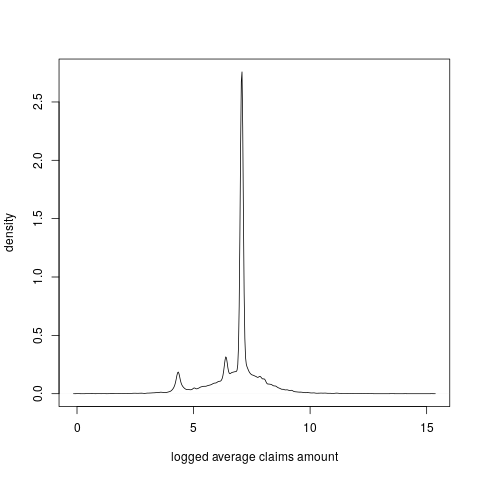
\includegraphics[width=0.4\linewidth]{../plots/sev/hist.png}
		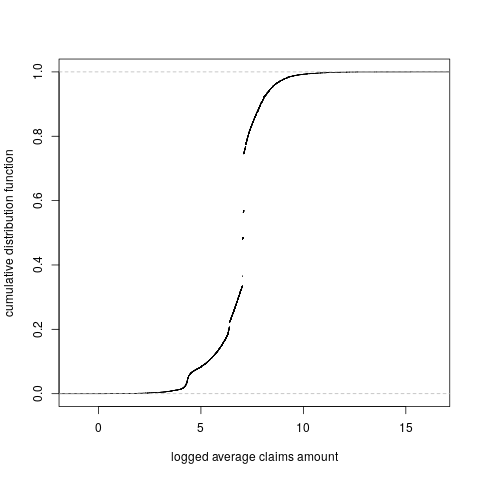
\includegraphics[width=0.4\linewidth]{../plots/sev/cdf.png}
		\caption{Histogram and the cumulative distribution function of logged average claims.}\label{hist}
	\end{figure}
An intuitive choice of component distributions is that 
three peaks are modeled by three gamma distributions, respectively, the resting non-tail part by a forth gamma distribution, and the tail part by a Pareto distribution.
Therefore, the probability density function (of the null model) is given by
\begin{equation}\label{sev-0}
	f(y|\bx;p,\mu,\phi,\alpha)=\sum_{k=1}^4p_kf_{G}(y;\mu_k,\phi_k)+p_5f_{P}(y;\alpha,M),
\end{equation}
	where $\mu,\phi$ are mean and dispersion parameter of gamma distribution, and $\alpha, M$ are tail index and threshold of Pareto distribution. 
	The logged survival function for logged average claims as shown in Figure \ref{tail} indicates a regularly varying  tail at infinity \citep{embrechts2013modelling}.
	The threshold of Pareto distribution is selected as $M=8158.13$ according to the Hill plot \citep{resnick1997heavy} as shown in Figure \ref{tail}. Please refer to \citet{wuthrich2022statistical} for more discussions on this data.
	
\begin{figure}[h!]
	\centering
	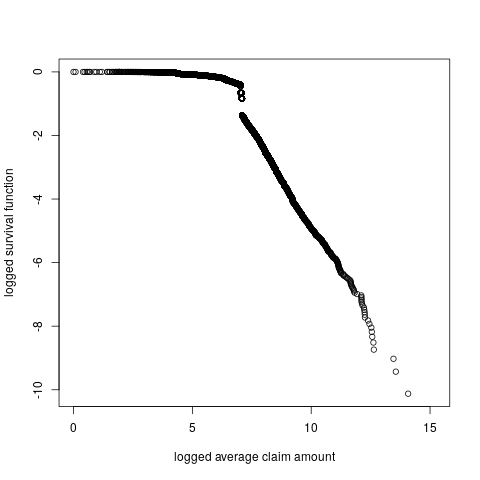
\includegraphics[width=0.4\linewidth]{../plots/sev/log-log.png}
	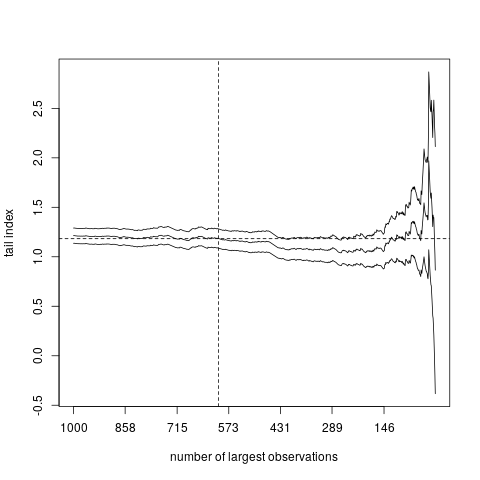
\includegraphics[width=0.4\linewidth]{../plots/sev/hill.png}
	\caption{The logged survival function and the Hill plot for logged average claims.}\label{tail}
\end{figure}
	
	The three peaks as shown in Figure \ref{hist} imply a way of initialization through the hidden component indicator variable:
	\begin{equation}
		\begin{aligned}
			\hat{\bz}^{[0]}_i&=(\hat{z}^{[0]}_{i,1},\hat{z}^{[0]}_{i,2},\hat{z}^{[0]}_{i,3},\hat{z}^{[0]}_{i,4},\hat{z}^{[0]}_{i,5})\\
			&=(\mathbbm{1}_{(0,500]}y_i,\mathbbm{1}_{(500, 1000]}y_i,\mathbbm{1}_{(1000,1200]}y_i,\mathbbm{1}_{(1200,8158.13]}y_i,\mathbbm{1}_{(8158.13,\infty)}y_i).
		\end{aligned}
	\end{equation}
	Component parameters $\mu,\phi,\alpha$ can be initialized as the MLEs in a homogeneous model for the full information $(y_i,\hat{\bz}_i^{[0]},\bx_i)_{i=1:n}$, i.e., the MLEs of parameters in gamma/Pareto distribution fitted to the partial samples in five intervals $(0,500], (500,1000], (1000,1200],(1200,8158.13],(8158.13,\infty)$, respectively.
	
We first fit a mixture of distributions \eqref{sev-0} to the data via the EM algorithm. 
The trace of learning loss is shown in Figure \ref{null_sev}, implying a convergence after 80 iterations.
	\begin{figure}[h!]
		\centering
		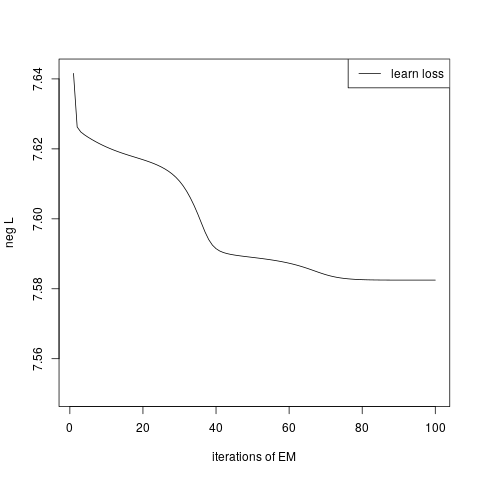
\includegraphics[width=0.4\linewidth]{../plots/sev/null_trace}
		\caption{The trace plot the learning loss for the homogeneous model \eqref{sev-0} during the EM iterations.}\label{null_sev}
	\end{figure}
The estimated component parameters are listed in Table \ref{null-gamma}. We observe that the three peaks are captured by the first three component gamma distributions.
	\begin{table}[h!]
		\centering
		\caption{The MLEs of component parameters in the homogeneous model \eqref{sev-0}. Tail index is estimated as $\hat{\alpha}=1.0773$.}\label{null-gamma}
		\begin{tabular}{crrrr}
			\hline
			component $k$ & \multicolumn{1}{c}{$\mu_k$} & \multicolumn{1}{c}{shape $(1/\phi_k)$} & \multicolumn{1}{c}{scale} & \multicolumn{1}{c}{rate} \\ \hline
			1         & 76.8727                & 105.556                   & 0.7283                    & 1.3731                   \\
			2         & 592.5909               & 653.539                   & 0.9067                    & 1.1029                   \\
			3         & 1171.3811              & 999.9999                  & 1.1714                    & 0.8537                   \\
			4         & 1534.5143              & 1.0377                    & 1478.7768                 & 7e-04                    \\ \hline
		\end{tabular}
	\end{table}
	The first three large shape parameters (small dispersion) imply the  difficulties with {mean modelling} in the first three component models.
	 The test loss is calculated as 7.5815. The mixing probabilities are estimated as $\hat{p}_1=0.0409,~ \hat{p}_2=0.0300, ~\hat{p}_3=0.4100,~ \hat{p}_4=0.4973$ and $\hat{p}_5=0.0218.$

Next we fit a mixture of distributions with heterogeneous mixing probabilities by the proposed EB algorithm:
\begin{equation}\label{sev-bst-p}
f(y|\bx;p,\mu,\phi,\alpha)=\sum_{k=1}^4p_k(\bx)f_{G}(y;\mu_k,\phi_k)+p_5(\bx)f_{P}(y;\alpha,M).
\end{equation}
We draw the boxplot of the mixing probabilities in Figure \ref{bx-bst-p}.
We observe that the mixing probabilities for the third and forth components $p_3$ and $p_4$ are more related with the covariates.
The test loss is calculated as 7.5588 smaller than the null model.
	\begin{figure}[htp!]
		\centering
		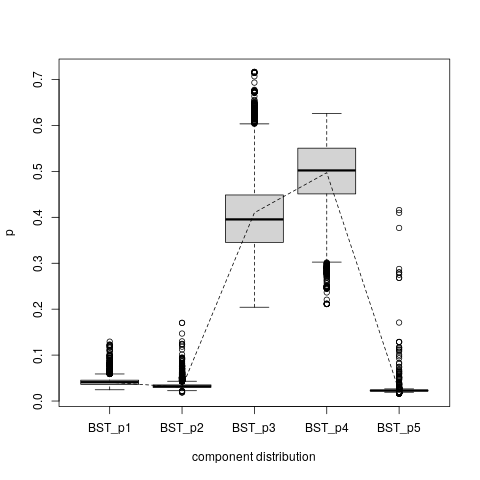
\includegraphics[width=0.35\linewidth]{../plots/sev/bst_p}
		\caption{The boxplot of the estimated mixing probabilities in Model \eqref{sev-bst-p}.}\label{bx-bst-p}
	\end{figure}


Finally, the small shape parameter of the forth component as shown in Table \ref{null-gamma} indicates a possible improvement by boosting the forth component  mean.
Therefore, we fit the following mixture model:
	$$
	\begin{aligned}
		f(y|\bx;p,\mu,\phi,\alpha)=&\sum_{k=1}^3p_k(\bx)f_{G}(y;\mu_k,\phi_k)+ \\
		&p_4(\bx)f_{G}(y|\bx;\mu_4(\bx),\phi_4)+ p_5(\bx)f_{P}(y;\alpha,M).
	\end{aligned}
	$$
	The test loss is calculated as 7.5573 slightly smaller than that for model \eqref{sev-bst-p}. 


\section{Conclusions}\label{sec:conclusions}
Insurance loss data sometimes cannot be sufficiently modeled by a single distribution, so a mixture of models is usually more preferred. Since there are multiple component models in a mixture of models, the parameter estimation problems is one key issue for data analysis. Thus, the EM algorithm is one critical estimation method for mixture models in the literature.
However, the EM algorithm usually requires parametric form of the component models, which limits the practical flexibility of mixture models.
In this paper, we propose an Expectation-Boosting (EB) algorithm for mixture models, where both the mixing probabilities and the component models can be modeled non-parametrically. 
The core of the proposed algorithm is to replace the maximization step of the EM algorithm with a generic functional gradient descent algorithm.
There are several advantages of the EB algorithm over the EM algorithm. 
First, boosting algorithm is a flexible non-parametric regression facilitating both {non-linear effects and interaction}.  
There is no need for specifying the form of component regression functions.
Automated feature engineering is performed during the EB algorithm.
Second, boosting algorithm is {overfitting-sensitive}, and {variable selection} is conducted simultaneously during the EB algorithm.
The cost of more flexibility is more computing time than the EM algorithm since there are several inner boosting loops in each EB iteration.{\color{blue}[I don't understand this sentence]}
We can accelerate the EB algorithm by conducting all the inner boosting loops simultaneously since they are independent given the component indicator variable $z$.
%In this paper, although we do not discuss model interpretation, the interpretation method in usual boosting algorithm can be implemented directly for mixture models such as variable importance, partial dependent plot, etc.

	\section*{Acknowledgment}
Guangyuan Gao gratefully acknowledges the financial support from the National Natural Science Foundation of China (71901207). Yanxi Hou gratefully acknowledges the financial support from the National Natural Science Foundation of China (72171055) and Natural Science Foundation of Shanghai (20ZR1403900).

\bibliography{boosting}
\bibliographystyle{boosting}

\end{document}
